\documentclass[twoside]{book}

% Packages required by doxygen
\usepackage{fixltx2e}
\usepackage{calc}
\usepackage{doxygen}
\usepackage[export]{adjustbox} % also loads graphicx
\usepackage{graphicx}
\usepackage[utf8]{inputenc}
\usepackage{makeidx}
\usepackage{multicol}
\usepackage{multirow}
\PassOptionsToPackage{warn}{textcomp}
\usepackage{textcomp}
\usepackage[nointegrals]{wasysym}
\usepackage[table]{xcolor}

% Font selection
\usepackage[T1]{fontenc}
\usepackage[scaled=.90]{helvet}
\usepackage{courier}
\usepackage{amssymb}
\usepackage{sectsty}
\renewcommand{\familydefault}{\sfdefault}
\allsectionsfont{%
  \fontseries{bc}\selectfont%
  \color{darkgray}%
}
\renewcommand{\DoxyLabelFont}{%
  \fontseries{bc}\selectfont%
  \color{darkgray}%
}
\newcommand{\+}{\discretionary{\mbox{\scriptsize$\hookleftarrow$}}{}{}}

% Page & text layout
\usepackage{geometry}
\geometry{%
  a4paper,%
  top=2.5cm,%
  bottom=2.5cm,%
  left=2.5cm,%
  right=2.5cm%
}
\tolerance=750
\hfuzz=15pt
\hbadness=750
\setlength{\emergencystretch}{15pt}
\setlength{\parindent}{0cm}
\setlength{\parskip}{3ex plus 2ex minus 2ex}
\makeatletter
\renewcommand{\paragraph}{%
  \@startsection{paragraph}{4}{0ex}{-1.0ex}{1.0ex}{%
    \normalfont\normalsize\bfseries\SS@parafont%
  }%
}
\renewcommand{\subparagraph}{%
  \@startsection{subparagraph}{5}{0ex}{-1.0ex}{1.0ex}{%
    \normalfont\normalsize\bfseries\SS@subparafont%
  }%
}
\makeatother

% Headers & footers
\usepackage{fancyhdr}
\pagestyle{fancyplain}
\fancyhead[LE]{\fancyplain{}{\bfseries\thepage}}
\fancyhead[CE]{\fancyplain{}{}}
\fancyhead[RE]{\fancyplain{}{\bfseries\leftmark}}
\fancyhead[LO]{\fancyplain{}{\bfseries\rightmark}}
\fancyhead[CO]{\fancyplain{}{}}
\fancyhead[RO]{\fancyplain{}{\bfseries\thepage}}
\fancyfoot[LE]{\fancyplain{}{}}
\fancyfoot[CE]{\fancyplain{}{}}
\fancyfoot[RE]{\fancyplain{}{\bfseries\scriptsize Generated by Doxygen }}
\fancyfoot[LO]{\fancyplain{}{\bfseries\scriptsize Generated by Doxygen }}
\fancyfoot[CO]{\fancyplain{}{}}
\fancyfoot[RO]{\fancyplain{}{}}
\renewcommand{\footrulewidth}{0.4pt}
\renewcommand{\chaptermark}[1]{%
  \markboth{#1}{}%
}
\renewcommand{\sectionmark}[1]{%
  \markright{\thesection\ #1}%
}

% Indices & bibliography
\usepackage{natbib}
\usepackage[titles]{tocloft}
\setcounter{tocdepth}{3}
\setcounter{secnumdepth}{5}
\makeindex

% Hyperlinks (required, but should be loaded last)
\usepackage{ifpdf}
\ifpdf
  \usepackage[pdftex,pagebackref=true]{hyperref}
\else
  \usepackage[ps2pdf,pagebackref=true]{hyperref}
\fi
\hypersetup{%
  colorlinks=true,%
  linkcolor=blue,%
  citecolor=blue,%
  unicode%
}

% Custom commands
\newcommand{\clearemptydoublepage}{%
  \newpage{\pagestyle{empty}\cleardoublepage}%
}

\usepackage{caption}
\captionsetup{labelsep=space,justification=centering,font={bf},singlelinecheck=off,skip=4pt,position=top}

%===== C O N T E N T S =====

\begin{document}

% Titlepage & ToC
\hypersetup{pageanchor=false,
             bookmarksnumbered=true,
             pdfencoding=unicode
            }
\pagenumbering{alph}
\begin{titlepage}
\vspace*{7cm}
\begin{center}%
{\Large cxx\+\_\+continued\+\_\+fractions }\\
\vspace*{1cm}
{\large Generated by Doxygen 1.8.13}\\
\end{center}
\end{titlepage}
\clearemptydoublepage
\pagenumbering{roman}
\tableofcontents
\clearemptydoublepage
\pagenumbering{arabic}
\hypersetup{pageanchor=true}

%--- Begin generated contents ---
\chapter{Class Index}
\section{Class List}
Here are the classes, structs, unions and interfaces with brief descriptions\+:\begin{DoxyCompactList}
\item\contentsline{section}{\hyperlink{struct____gnu__cxx_1_1____airy__t}{\+\_\+\+\_\+gnu\+\_\+cxx\+::\+\_\+\+\_\+airy\+\_\+t$<$ \+\_\+\+Tx, \+\_\+\+Tp $>$} }{\pageref{struct____gnu__cxx_1_1____airy__t}}{}
\item\contentsline{section}{\hyperlink{struct____gnu__cxx_1_1____cyl__bessel__t}{\+\_\+\+\_\+gnu\+\_\+cxx\+::\+\_\+\+\_\+cyl\+\_\+bessel\+\_\+t$<$ \+\_\+\+Tnu, \+\_\+\+Tx, \+\_\+\+Tp $>$} }{\pageref{struct____gnu__cxx_1_1____cyl__bessel__t}}{}
\item\contentsline{section}{\hyperlink{struct____gnu__cxx_1_1____cyl__hankel__t}{\+\_\+\+\_\+gnu\+\_\+cxx\+::\+\_\+\+\_\+cyl\+\_\+hankel\+\_\+t$<$ \+\_\+\+Tnu, \+\_\+\+Tx, \+\_\+\+Tp $>$} }{\pageref{struct____gnu__cxx_1_1____cyl__hankel__t}}{}
\item\contentsline{section}{\hyperlink{struct____gnu__cxx_1_1____cyl__mod__bessel__t}{\+\_\+\+\_\+gnu\+\_\+cxx\+::\+\_\+\+\_\+cyl\+\_\+mod\+\_\+bessel\+\_\+t$<$ \+\_\+\+Tnu, \+\_\+\+Tx, \+\_\+\+Tp $>$} }{\pageref{struct____gnu__cxx_1_1____cyl__mod__bessel__t}}{}
\item\contentsline{section}{\hyperlink{struct____gnu__cxx_1_1____fock__airy__t}{\+\_\+\+\_\+gnu\+\_\+cxx\+::\+\_\+\+\_\+fock\+\_\+airy\+\_\+t$<$ \+\_\+\+Tx, \+\_\+\+Tp $>$} }{\pageref{struct____gnu__cxx_1_1____fock__airy__t}}{}
\item\contentsline{section}{\hyperlink{struct____gnu__cxx_1_1____fp__is__integer__t}{\+\_\+\+\_\+gnu\+\_\+cxx\+::\+\_\+\+\_\+fp\+\_\+is\+\_\+integer\+\_\+t} }{\pageref{struct____gnu__cxx_1_1____fp__is__integer__t}}{}
\item\contentsline{section}{\hyperlink{struct____gnu__cxx_1_1____gamma__inc__t}{\+\_\+\+\_\+gnu\+\_\+cxx\+::\+\_\+\+\_\+gamma\+\_\+inc\+\_\+t$<$ \+\_\+\+Tp $>$} }{\pageref{struct____gnu__cxx_1_1____gamma__inc__t}}{}
\item\contentsline{section}{\hyperlink{struct____gnu__cxx_1_1____gamma__temme__t}{\+\_\+\+\_\+gnu\+\_\+cxx\+::\+\_\+\+\_\+gamma\+\_\+temme\+\_\+t$<$ \+\_\+\+Tp $>$} \\*A structure for the gamma functions required by the Temme series expansions of $ N_\nu(x) $ and $ K_\nu(x) $. \[ \Gamma_1 = \frac{1}{2\mu} \left[\frac{1}{\Gamma(1 - \mu)} - \frac{1}{\Gamma(1 + \mu)}\right] \] and \[ \Gamma_2 = \frac{1}{2} \left[\frac{1}{\Gamma(1 - \mu)} + \frac{1}{\Gamma(1 + \mu)}\right] \] where $ -1/2 <= \mu <= 1/2 $ is $ \mu = \nu - N $ and $ N $. is the nearest integer to $ \nu $. The values of $ \Gamma(1 + \mu) $ and $ \Gamma(1 - \mu) $ are returned as well }{\pageref{struct____gnu__cxx_1_1____gamma__temme__t}}{}
\item\contentsline{section}{\hyperlink{struct____gnu__cxx_1_1____jacobi__t}{\+\_\+\+\_\+gnu\+\_\+cxx\+::\+\_\+\+\_\+jacobi\+\_\+t$<$ \+\_\+\+Tp $>$} }{\pageref{struct____gnu__cxx_1_1____jacobi__t}}{}
\item\contentsline{section}{\hyperlink{struct____gnu__cxx_1_1____lgamma__t}{\+\_\+\+\_\+gnu\+\_\+cxx\+::\+\_\+\+\_\+lgamma\+\_\+t$<$ \+\_\+\+Tp $>$} }{\pageref{struct____gnu__cxx_1_1____lgamma__t}}{}
\item\contentsline{section}{\hyperlink{struct____gnu__cxx_1_1____pqgamma__t}{\+\_\+\+\_\+gnu\+\_\+cxx\+::\+\_\+\+\_\+pqgamma\+\_\+t$<$ \+\_\+\+Tp $>$} }{\pageref{struct____gnu__cxx_1_1____pqgamma__t}}{}
\item\contentsline{section}{\hyperlink{struct____gnu__cxx_1_1____quadrature__point__t}{\+\_\+\+\_\+gnu\+\_\+cxx\+::\+\_\+\+\_\+quadrature\+\_\+point\+\_\+t$<$ \+\_\+\+Tp $>$} }{\pageref{struct____gnu__cxx_1_1____quadrature__point__t}}{}
\item\contentsline{section}{\hyperlink{struct____gnu__cxx_1_1____sincos__t}{\+\_\+\+\_\+gnu\+\_\+cxx\+::\+\_\+\+\_\+sincos\+\_\+t$<$ \+\_\+\+Tp $>$} }{\pageref{struct____gnu__cxx_1_1____sincos__t}}{}
\item\contentsline{section}{\hyperlink{struct____gnu__cxx_1_1____sph__bessel__t}{\+\_\+\+\_\+gnu\+\_\+cxx\+::\+\_\+\+\_\+sph\+\_\+bessel\+\_\+t$<$ \+\_\+\+Tn, \+\_\+\+Tx, \+\_\+\+Tp $>$} }{\pageref{struct____gnu__cxx_1_1____sph__bessel__t}}{}
\item\contentsline{section}{\hyperlink{struct____gnu__cxx_1_1____sph__hankel__t}{\+\_\+\+\_\+gnu\+\_\+cxx\+::\+\_\+\+\_\+sph\+\_\+hankel\+\_\+t$<$ \+\_\+\+Tn, \+\_\+\+Tx, \+\_\+\+Tp $>$} }{\pageref{struct____gnu__cxx_1_1____sph__hankel__t}}{}
\item\contentsline{section}{\hyperlink{struct____gnu__cxx_1_1____sph__mod__bessel__t}{\+\_\+\+\_\+gnu\+\_\+cxx\+::\+\_\+\+\_\+sph\+\_\+mod\+\_\+bessel\+\_\+t$<$ \+\_\+\+Tn, \+\_\+\+Tx, \+\_\+\+Tp $>$} }{\pageref{struct____gnu__cxx_1_1____sph__mod__bessel__t}}{}
\item\contentsline{section}{\hyperlink{structstd_1_1____detail_1_1____gamma__lanczos__data}{std\+::\+\_\+\+\_\+detail\+::\+\_\+\+\_\+gamma\+\_\+lanczos\+\_\+data$<$ \+\_\+\+Tp $>$} }{\pageref{structstd_1_1____detail_1_1____gamma__lanczos__data}}{}
\item\contentsline{section}{\hyperlink{structstd_1_1____detail_1_1____gamma__lanczos__data_3_01double_01_4}{std\+::\+\_\+\+\_\+detail\+::\+\_\+\+\_\+gamma\+\_\+lanczos\+\_\+data$<$ double $>$} }{\pageref{structstd_1_1____detail_1_1____gamma__lanczos__data_3_01double_01_4}}{}
\item\contentsline{section}{\hyperlink{structstd_1_1____detail_1_1____gamma__lanczos__data_3_01float_01_4}{std\+::\+\_\+\+\_\+detail\+::\+\_\+\+\_\+gamma\+\_\+lanczos\+\_\+data$<$ float $>$} }{\pageref{structstd_1_1____detail_1_1____gamma__lanczos__data_3_01float_01_4}}{}
\item\contentsline{section}{\hyperlink{structstd_1_1____detail_1_1____gamma__lanczos__data_3_01long_01double_01_4}{std\+::\+\_\+\+\_\+detail\+::\+\_\+\+\_\+gamma\+\_\+lanczos\+\_\+data$<$ long double $>$} }{\pageref{structstd_1_1____detail_1_1____gamma__lanczos__data_3_01long_01double_01_4}}{}
\item\contentsline{section}{\hyperlink{structstd_1_1____detail_1_1____gamma__spouge__data}{std\+::\+\_\+\+\_\+detail\+::\+\_\+\+\_\+gamma\+\_\+spouge\+\_\+data$<$ \+\_\+\+Tp $>$} }{\pageref{structstd_1_1____detail_1_1____gamma__spouge__data}}{}
\item\contentsline{section}{\hyperlink{structstd_1_1____detail_1_1____gamma__spouge__data_3_01double_01_4}{std\+::\+\_\+\+\_\+detail\+::\+\_\+\+\_\+gamma\+\_\+spouge\+\_\+data$<$ double $>$} }{\pageref{structstd_1_1____detail_1_1____gamma__spouge__data_3_01double_01_4}}{}
\item\contentsline{section}{\hyperlink{structstd_1_1____detail_1_1____gamma__spouge__data_3_01float_01_4}{std\+::\+\_\+\+\_\+detail\+::\+\_\+\+\_\+gamma\+\_\+spouge\+\_\+data$<$ float $>$} }{\pageref{structstd_1_1____detail_1_1____gamma__spouge__data_3_01float_01_4}}{}
\item\contentsline{section}{\hyperlink{structstd_1_1____detail_1_1____gamma__spouge__data_3_01long_01double_01_4}{std\+::\+\_\+\+\_\+detail\+::\+\_\+\+\_\+gamma\+\_\+spouge\+\_\+data$<$ long double $>$} }{\pageref{structstd_1_1____detail_1_1____gamma__spouge__data_3_01long_01double_01_4}}{}
\item\contentsline{section}{\hyperlink{classstd_1_1____detail_1_1__Airy}{std\+::\+\_\+\+\_\+detail\+::\+\_\+\+Airy$<$ \+\_\+\+Tp $>$} }{\pageref{classstd_1_1____detail_1_1__Airy}}{}
\item\contentsline{section}{\hyperlink{classstd_1_1____detail_1_1__Airy__asymp}{std\+::\+\_\+\+\_\+detail\+::\+\_\+\+Airy\+\_\+asymp$<$ \+\_\+\+Tp $>$} }{\pageref{classstd_1_1____detail_1_1__Airy__asymp}}{}
\item\contentsline{section}{\hyperlink{structstd_1_1____detail_1_1__Airy__asymp__data}{std\+::\+\_\+\+\_\+detail\+::\+\_\+\+Airy\+\_\+asymp\+\_\+data$<$ \+\_\+\+Tp $>$} }{\pageref{structstd_1_1____detail_1_1__Airy__asymp__data}}{}
\item\contentsline{section}{\hyperlink{structstd_1_1____detail_1_1__Airy__asymp__data_3_01double_01_4}{std\+::\+\_\+\+\_\+detail\+::\+\_\+\+Airy\+\_\+asymp\+\_\+data$<$ double $>$} }{\pageref{structstd_1_1____detail_1_1__Airy__asymp__data_3_01double_01_4}}{}
\item\contentsline{section}{\hyperlink{structstd_1_1____detail_1_1__Airy__asymp__data_3_01float_01_4}{std\+::\+\_\+\+\_\+detail\+::\+\_\+\+Airy\+\_\+asymp\+\_\+data$<$ float $>$} }{\pageref{structstd_1_1____detail_1_1__Airy__asymp__data_3_01float_01_4}}{}
\item\contentsline{section}{\hyperlink{structstd_1_1____detail_1_1__Airy__asymp__data_3_01long_01double_01_4}{std\+::\+\_\+\+\_\+detail\+::\+\_\+\+Airy\+\_\+asymp\+\_\+data$<$ long double $>$} }{\pageref{structstd_1_1____detail_1_1__Airy__asymp__data_3_01long_01double_01_4}}{}
\item\contentsline{section}{\hyperlink{classstd_1_1____detail_1_1__Airy__asymp__series}{std\+::\+\_\+\+\_\+detail\+::\+\_\+\+Airy\+\_\+asymp\+\_\+series$<$ \+\_\+\+Sum $>$} }{\pageref{classstd_1_1____detail_1_1__Airy__asymp__series}}{}
\item\contentsline{section}{\hyperlink{structstd_1_1____detail_1_1__Airy__default__radii}{std\+::\+\_\+\+\_\+detail\+::\+\_\+\+Airy\+\_\+default\+\_\+radii$<$ \+\_\+\+Tp $>$} }{\pageref{structstd_1_1____detail_1_1__Airy__default__radii}}{}
\item\contentsline{section}{\hyperlink{structstd_1_1____detail_1_1__Airy__default__radii_3_01double_01_4}{std\+::\+\_\+\+\_\+detail\+::\+\_\+\+Airy\+\_\+default\+\_\+radii$<$ double $>$} }{\pageref{structstd_1_1____detail_1_1__Airy__default__radii_3_01double_01_4}}{}
\item\contentsline{section}{\hyperlink{structstd_1_1____detail_1_1__Airy__default__radii_3_01float_01_4}{std\+::\+\_\+\+\_\+detail\+::\+\_\+\+Airy\+\_\+default\+\_\+radii$<$ float $>$} }{\pageref{structstd_1_1____detail_1_1__Airy__default__radii_3_01float_01_4}}{}
\item\contentsline{section}{\hyperlink{structstd_1_1____detail_1_1__Airy__default__radii_3_01long_01double_01_4}{std\+::\+\_\+\+\_\+detail\+::\+\_\+\+Airy\+\_\+default\+\_\+radii$<$ long double $>$} }{\pageref{structstd_1_1____detail_1_1__Airy__default__radii_3_01long_01double_01_4}}{}
\item\contentsline{section}{\hyperlink{classstd_1_1____detail_1_1__Airy__series}{std\+::\+\_\+\+\_\+detail\+::\+\_\+\+Airy\+\_\+series$<$ \+\_\+\+Tp $>$} }{\pageref{classstd_1_1____detail_1_1__Airy__series}}{}
\item\contentsline{section}{\hyperlink{structstd_1_1____detail_1_1__AiryAuxilliaryState}{std\+::\+\_\+\+\_\+detail\+::\+\_\+\+Airy\+Auxilliary\+State$<$ \+\_\+\+Tp $>$} }{\pageref{structstd_1_1____detail_1_1__AiryAuxilliaryState}}{}
\item\contentsline{section}{\hyperlink{structstd_1_1____detail_1_1__AiryState}{std\+::\+\_\+\+\_\+detail\+::\+\_\+\+Airy\+State$<$ \+\_\+\+Tp $>$} }{\pageref{structstd_1_1____detail_1_1__AiryState}}{}
\item\contentsline{section}{\hyperlink{structstd_1_1____detail_1_1__Factorial__table}{std\+::\+\_\+\+\_\+detail\+::\+\_\+\+Factorial\+\_\+table$<$ \+\_\+\+Tp $>$} }{\pageref{structstd_1_1____detail_1_1__Factorial__table}}{}
\end{DoxyCompactList}

\chapter{File Index}
\section{File List}
Here is a list of all files with brief descriptions\+:\begin{DoxyCompactList}
\item\contentsline{section}{bits/\hyperlink{sf__airy_8tcc}{sf\+\_\+airy.\+tcc} }{\pageref{sf__airy_8tcc}}{}
\item\contentsline{section}{bits/\hyperlink{sf__bernoulli_8tcc}{sf\+\_\+bernoulli.\+tcc} }{\pageref{sf__bernoulli_8tcc}}{}
\item\contentsline{section}{bits/\hyperlink{sf__bessel_8tcc}{sf\+\_\+bessel.\+tcc} }{\pageref{sf__bessel_8tcc}}{}
\item\contentsline{section}{bits/\hyperlink{sf__beta_8tcc}{sf\+\_\+beta.\+tcc} }{\pageref{sf__beta_8tcc}}{}
\item\contentsline{section}{bits/\hyperlink{sf__cardinal_8tcc}{sf\+\_\+cardinal.\+tcc} }{\pageref{sf__cardinal_8tcc}}{}
\item\contentsline{section}{bits/\hyperlink{sf__chebyshev_8tcc}{sf\+\_\+chebyshev.\+tcc} }{\pageref{sf__chebyshev_8tcc}}{}
\item\contentsline{section}{bits/\hyperlink{sf__coulomb_8tcc}{sf\+\_\+coulomb.\+tcc} }{\pageref{sf__coulomb_8tcc}}{}
\item\contentsline{section}{bits/\hyperlink{sf__dawson_8tcc}{sf\+\_\+dawson.\+tcc} }{\pageref{sf__dawson_8tcc}}{}
\item\contentsline{section}{bits/\hyperlink{sf__distributions_8tcc}{sf\+\_\+distributions.\+tcc} }{\pageref{sf__distributions_8tcc}}{}
\item\contentsline{section}{bits/\hyperlink{sf__ellint_8tcc}{sf\+\_\+ellint.\+tcc} }{\pageref{sf__ellint_8tcc}}{}
\item\contentsline{section}{bits/\hyperlink{sf__euler_8tcc}{sf\+\_\+euler.\+tcc} }{\pageref{sf__euler_8tcc}}{}
\item\contentsline{section}{bits/\hyperlink{sf__expint_8tcc}{sf\+\_\+expint.\+tcc} }{\pageref{sf__expint_8tcc}}{}
\item\contentsline{section}{bits/\hyperlink{sf__fresnel_8tcc}{sf\+\_\+fresnel.\+tcc} }{\pageref{sf__fresnel_8tcc}}{}
\item\contentsline{section}{bits/\hyperlink{sf__gamma_8tcc}{sf\+\_\+gamma.\+tcc} }{\pageref{sf__gamma_8tcc}}{}
\item\contentsline{section}{bits/\hyperlink{sf__gegenbauer_8tcc}{sf\+\_\+gegenbauer.\+tcc} }{\pageref{sf__gegenbauer_8tcc}}{}
\item\contentsline{section}{bits/\hyperlink{sf__hankel_8tcc}{sf\+\_\+hankel.\+tcc} }{\pageref{sf__hankel_8tcc}}{}
\item\contentsline{section}{bits/\hyperlink{sf__hermite_8tcc}{sf\+\_\+hermite.\+tcc} }{\pageref{sf__hermite_8tcc}}{}
\item\contentsline{section}{bits/\hyperlink{sf__hyperg_8tcc}{sf\+\_\+hyperg.\+tcc} }{\pageref{sf__hyperg_8tcc}}{}
\item\contentsline{section}{bits/\hyperlink{sf__hypint_8tcc}{sf\+\_\+hypint.\+tcc} }{\pageref{sf__hypint_8tcc}}{}
\item\contentsline{section}{bits/\hyperlink{sf__jacobi_8tcc}{sf\+\_\+jacobi.\+tcc} }{\pageref{sf__jacobi_8tcc}}{}
\item\contentsline{section}{bits/\hyperlink{sf__laguerre_8tcc}{sf\+\_\+laguerre.\+tcc} }{\pageref{sf__laguerre_8tcc}}{}
\item\contentsline{section}{bits/\hyperlink{sf__legendre_8tcc}{sf\+\_\+legendre.\+tcc} }{\pageref{sf__legendre_8tcc}}{}
\item\contentsline{section}{bits/\hyperlink{sf__mod__bessel_8tcc}{sf\+\_\+mod\+\_\+bessel.\+tcc} }{\pageref{sf__mod__bessel_8tcc}}{}
\item\contentsline{section}{bits/\hyperlink{sf__owens__t_8tcc}{sf\+\_\+owens\+\_\+t.\+tcc} }{\pageref{sf__owens__t_8tcc}}{}
\item\contentsline{section}{bits/\hyperlink{sf__polylog_8tcc}{sf\+\_\+polylog.\+tcc} }{\pageref{sf__polylog_8tcc}}{}
\item\contentsline{section}{bits/\hyperlink{sf__stirling_8tcc}{sf\+\_\+stirling.\+tcc} }{\pageref{sf__stirling_8tcc}}{}
\item\contentsline{section}{bits/\hyperlink{sf__theta_8tcc}{sf\+\_\+theta.\+tcc} }{\pageref{sf__theta_8tcc}}{}
\item\contentsline{section}{bits/\hyperlink{sf__trig_8tcc}{sf\+\_\+trig.\+tcc} }{\pageref{sf__trig_8tcc}}{}
\item\contentsline{section}{bits/\hyperlink{sf__trigint_8tcc}{sf\+\_\+trigint.\+tcc} }{\pageref{sf__trigint_8tcc}}{}
\item\contentsline{section}{bits/\hyperlink{sf__zeta_8tcc}{sf\+\_\+zeta.\+tcc} }{\pageref{sf__zeta_8tcc}}{}
\item\contentsline{section}{bits/\hyperlink{specfun_8h}{specfun.\+h} }{\pageref{specfun_8h}}{}
\item\contentsline{section}{bits/\hyperlink{specfun__state_8h}{specfun\+\_\+state.\+h} }{\pageref{specfun__state_8h}}{}
\item\contentsline{section}{ext/\hyperlink{math__util_8h}{math\+\_\+util.\+h} }{\pageref{math__util_8h}}{}
\end{DoxyCompactList}

\chapter{Class Documentation}
\hypertarget{class__ForwardContinuedFraction}{}\section{\+\_\+\+Forward\+Continued\+Fraction$<$ \+\_\+\+Tp, \+\_\+\+A\+Fun, \+\_\+\+B\+Fun, \+\_\+\+Tail\+Fun $>$ Class Template Reference}
\label{class__ForwardContinuedFraction}\index{\+\_\+\+Forward\+Continued\+Fraction$<$ \+\_\+\+Tp, \+\_\+\+A\+Fun, \+\_\+\+B\+Fun, \+\_\+\+Tail\+Fun $>$@{\+\_\+\+Forward\+Continued\+Fraction$<$ \+\_\+\+Tp, \+\_\+\+A\+Fun, \+\_\+\+B\+Fun, \+\_\+\+Tail\+Fun $>$}}
\subsection*{Public Types}
\begin{DoxyCompactItemize}
\item 
using \hyperlink{class__ForwardContinuedFraction_aa3cd354821d01eff12c24f0c4283b6ee}{\+\_\+\+A\+Ret} = decltype(\+\_\+\+M\+\_\+num(0ull, \+\_\+\+Tp\{\}))
\item 
using \hyperlink{class__ForwardContinuedFraction_a0353d4790204b04fca698a26fa9a7d0b}{\+\_\+\+B\+Ret} = decltype(\+\_\+\+M\+\_\+den(0ull, \+\_\+\+Tp\{\}))
\item 
using \hyperlink{class__ForwardContinuedFraction_ab67bebe1ce3d9ab53ac76024af1b2007}{\+\_\+\+Ret} = decltype(\hyperlink{class__ForwardContinuedFraction_aa3cd354821d01eff12c24f0c4283b6ee}{\+\_\+\+A\+Ret}(0, \+\_\+\+Tp\{\})/\hyperlink{class__ForwardContinuedFraction_a0353d4790204b04fca698a26fa9a7d0b}{\+\_\+\+B\+Ret}(0, \+\_\+\+Tp\{\}))
\end{DoxyCompactItemize}
\subsection*{Public Member Functions}
\begin{DoxyCompactItemize}
\item 
\hyperlink{class__ForwardContinuedFraction_a0337894d9199abad9dbbfba007cf3dbd}{\+\_\+\+Forward\+Continued\+Fraction} (\+\_\+\+A\+Fun \+\_\+\+\_\+a, \+\_\+\+B\+Fun \+\_\+\+\_\+b, \+\_\+\+Tail\+Fun \+\_\+\+\_\+w)
\item 
\hyperlink{class__ForwardContinuedFraction_ab67bebe1ce3d9ab53ac76024af1b2007}{\+\_\+\+Ret} \hyperlink{class__ForwardContinuedFraction_a6fb6032d848099b493b23b8453fcb5e1}{operator()} (\+\_\+\+Tp \+\_\+\+\_\+x) const
\end{DoxyCompactItemize}


\subsection{Detailed Description}
\subsubsection*{template$<$typename \+\_\+\+Tp, typename \+\_\+\+A\+Fun, typename \+\_\+\+B\+Fun, typename \+\_\+\+Tail\+Fun$>$\newline
class \+\_\+\+Forward\+Continued\+Fraction$<$ \+\_\+\+Tp, \+\_\+\+A\+Fun, \+\_\+\+B\+Fun, \+\_\+\+Tail\+Fun $>$}

You need a functor belching a, b an iterator pair for a and an iterator for b 

\subsection{Member Typedef Documentation}
\mbox{\Hypertarget{class__ForwardContinuedFraction_aa3cd354821d01eff12c24f0c4283b6ee}\label{class__ForwardContinuedFraction_aa3cd354821d01eff12c24f0c4283b6ee}} 
\index{\+\_\+\+Forward\+Continued\+Fraction@{\+\_\+\+Forward\+Continued\+Fraction}!\+\_\+\+A\+Ret@{\+\_\+\+A\+Ret}}
\index{\+\_\+\+A\+Ret@{\+\_\+\+A\+Ret}!\+\_\+\+Forward\+Continued\+Fraction@{\+\_\+\+Forward\+Continued\+Fraction}}
\subsubsection{\texorpdfstring{\+\_\+\+A\+Ret}{\_ARet}}
{\footnotesize\ttfamily template$<$typename \+\_\+\+Tp , typename \+\_\+\+A\+Fun , typename \+\_\+\+B\+Fun , typename \+\_\+\+Tail\+Fun $>$ \\
using \hyperlink{class__ForwardContinuedFraction}{\+\_\+\+Forward\+Continued\+Fraction}$<$ \+\_\+\+Tp, \+\_\+\+A\+Fun, \+\_\+\+B\+Fun, \+\_\+\+Tail\+Fun $>$\+::\hyperlink{class__ForwardContinuedFraction_aa3cd354821d01eff12c24f0c4283b6ee}{\+\_\+\+A\+Ret} =  decltype(\+\_\+\+M\+\_\+num(0ull, \+\_\+\+Tp\{\}))}

\mbox{\Hypertarget{class__ForwardContinuedFraction_a0353d4790204b04fca698a26fa9a7d0b}\label{class__ForwardContinuedFraction_a0353d4790204b04fca698a26fa9a7d0b}} 
\index{\+\_\+\+Forward\+Continued\+Fraction@{\+\_\+\+Forward\+Continued\+Fraction}!\+\_\+\+B\+Ret@{\+\_\+\+B\+Ret}}
\index{\+\_\+\+B\+Ret@{\+\_\+\+B\+Ret}!\+\_\+\+Forward\+Continued\+Fraction@{\+\_\+\+Forward\+Continued\+Fraction}}
\subsubsection{\texorpdfstring{\+\_\+\+B\+Ret}{\_BRet}}
{\footnotesize\ttfamily template$<$typename \+\_\+\+Tp , typename \+\_\+\+A\+Fun , typename \+\_\+\+B\+Fun , typename \+\_\+\+Tail\+Fun $>$ \\
using \hyperlink{class__ForwardContinuedFraction}{\+\_\+\+Forward\+Continued\+Fraction}$<$ \+\_\+\+Tp, \+\_\+\+A\+Fun, \+\_\+\+B\+Fun, \+\_\+\+Tail\+Fun $>$\+::\hyperlink{class__ForwardContinuedFraction_a0353d4790204b04fca698a26fa9a7d0b}{\+\_\+\+B\+Ret} =  decltype(\+\_\+\+M\+\_\+den(0ull, \+\_\+\+Tp\{\}))}

\mbox{\Hypertarget{class__ForwardContinuedFraction_ab67bebe1ce3d9ab53ac76024af1b2007}\label{class__ForwardContinuedFraction_ab67bebe1ce3d9ab53ac76024af1b2007}} 
\index{\+\_\+\+Forward\+Continued\+Fraction@{\+\_\+\+Forward\+Continued\+Fraction}!\+\_\+\+Ret@{\+\_\+\+Ret}}
\index{\+\_\+\+Ret@{\+\_\+\+Ret}!\+\_\+\+Forward\+Continued\+Fraction@{\+\_\+\+Forward\+Continued\+Fraction}}
\subsubsection{\texorpdfstring{\+\_\+\+Ret}{\_Ret}}
{\footnotesize\ttfamily template$<$typename \+\_\+\+Tp , typename \+\_\+\+A\+Fun , typename \+\_\+\+B\+Fun , typename \+\_\+\+Tail\+Fun $>$ \\
using \hyperlink{class__ForwardContinuedFraction}{\+\_\+\+Forward\+Continued\+Fraction}$<$ \+\_\+\+Tp, \+\_\+\+A\+Fun, \+\_\+\+B\+Fun, \+\_\+\+Tail\+Fun $>$\+::\hyperlink{class__ForwardContinuedFraction_ab67bebe1ce3d9ab53ac76024af1b2007}{\+\_\+\+Ret} =  decltype(\hyperlink{class__ForwardContinuedFraction_aa3cd354821d01eff12c24f0c4283b6ee}{\+\_\+\+A\+Ret}(0, \+\_\+\+Tp\{\}) / \hyperlink{class__ForwardContinuedFraction_a0353d4790204b04fca698a26fa9a7d0b}{\+\_\+\+B\+Ret}(0, \+\_\+\+Tp\{\}))}



\subsection{Constructor \& Destructor Documentation}
\mbox{\Hypertarget{class__ForwardContinuedFraction_a0337894d9199abad9dbbfba007cf3dbd}\label{class__ForwardContinuedFraction_a0337894d9199abad9dbbfba007cf3dbd}} 
\index{\+\_\+\+Forward\+Continued\+Fraction@{\+\_\+\+Forward\+Continued\+Fraction}!\+\_\+\+Forward\+Continued\+Fraction@{\+\_\+\+Forward\+Continued\+Fraction}}
\index{\+\_\+\+Forward\+Continued\+Fraction@{\+\_\+\+Forward\+Continued\+Fraction}!\+\_\+\+Forward\+Continued\+Fraction@{\+\_\+\+Forward\+Continued\+Fraction}}
\subsubsection{\texorpdfstring{\+\_\+\+Forward\+Continued\+Fraction()}{\_ForwardContinuedFraction()}}
{\footnotesize\ttfamily template$<$typename \+\_\+\+Tp , typename \+\_\+\+A\+Fun , typename \+\_\+\+B\+Fun , typename \+\_\+\+Tail\+Fun $>$ \\
\hyperlink{class__ForwardContinuedFraction}{\+\_\+\+Forward\+Continued\+Fraction}$<$ \+\_\+\+Tp, \+\_\+\+A\+Fun, \+\_\+\+B\+Fun, \+\_\+\+Tail\+Fun $>$\+::\hyperlink{class__ForwardContinuedFraction}{\+\_\+\+Forward\+Continued\+Fraction} (\begin{DoxyParamCaption}\item[{\+\_\+\+A\+Fun}]{\+\_\+\+\_\+a,  }\item[{\+\_\+\+B\+Fun}]{\+\_\+\+\_\+b,  }\item[{\+\_\+\+Tail\+Fun}]{\+\_\+\+\_\+w }\end{DoxyParamCaption})\hspace{0.3cm}{\ttfamily [inline]}}



\subsection{Member Function Documentation}
\mbox{\Hypertarget{class__ForwardContinuedFraction_a6fb6032d848099b493b23b8453fcb5e1}\label{class__ForwardContinuedFraction_a6fb6032d848099b493b23b8453fcb5e1}} 
\index{\+\_\+\+Forward\+Continued\+Fraction@{\+\_\+\+Forward\+Continued\+Fraction}!operator()@{operator()}}
\index{operator()@{operator()}!\+\_\+\+Forward\+Continued\+Fraction@{\+\_\+\+Forward\+Continued\+Fraction}}
\subsubsection{\texorpdfstring{operator()()}{operator()()}}
{\footnotesize\ttfamily template$<$typename \+\_\+\+Tp , typename \+\_\+\+A\+Fun , typename \+\_\+\+B\+Fun , typename \+\_\+\+Tail\+Fun $>$ \\
\hyperlink{class__ForwardContinuedFraction_ab67bebe1ce3d9ab53ac76024af1b2007}{\+\_\+\+Ret} \hyperlink{class__ForwardContinuedFraction}{\+\_\+\+Forward\+Continued\+Fraction}$<$ \+\_\+\+Tp, \+\_\+\+A\+Fun, \+\_\+\+B\+Fun, \+\_\+\+Tail\+Fun $>$\+::operator() (\begin{DoxyParamCaption}\item[{\+\_\+\+Tp}]{\+\_\+\+\_\+x }\end{DoxyParamCaption}) const\hspace{0.3cm}{\ttfamily [inline]}}



The documentation for this class was generated from the following file\+:\begin{DoxyCompactItemize}
\item 
include/ext/\hyperlink{cfrac__forward_8tcc}{cfrac\+\_\+forward.\+tcc}\end{DoxyCompactItemize}

\hypertarget{class__LentzContinuedFraction}{}\section{\+\_\+\+Lentz\+Continued\+Fraction$<$ \+\_\+\+Tp, \+\_\+\+A\+Fun, \+\_\+\+B\+Fun, \+\_\+\+Tail\+Fun $>$ Class Template Reference}
\label{class__LentzContinuedFraction}\index{\+\_\+\+Lentz\+Continued\+Fraction$<$ \+\_\+\+Tp, \+\_\+\+A\+Fun, \+\_\+\+B\+Fun, \+\_\+\+Tail\+Fun $>$@{\+\_\+\+Lentz\+Continued\+Fraction$<$ \+\_\+\+Tp, \+\_\+\+A\+Fun, \+\_\+\+B\+Fun, \+\_\+\+Tail\+Fun $>$}}
\subsection*{Public Types}
\begin{DoxyCompactItemize}
\item 
using \hyperlink{class__LentzContinuedFraction_a44dee6f8bd3dfe70d76c85b518589dec}{\+\_\+\+A\+Ret} = decltype(\+\_\+\+M\+\_\+num(0ull, \+\_\+\+Tp\{\}))
\item 
using \hyperlink{class__LentzContinuedFraction_a97536abf4c68ac813d692d204ac47ba4}{\+\_\+\+B\+Ret} = decltype(\+\_\+\+M\+\_\+den(0ull, \+\_\+\+Tp\{\}))
\item 
using \hyperlink{class__LentzContinuedFraction_ae549d8853f57a08201bea3a926d30992}{\+\_\+\+Ret} = decltype(\+\_\+\+M\+\_\+num(0ull, \+\_\+\+Tp\{\})/\+\_\+\+M\+\_\+den(0ull, \+\_\+\+Tp\{\}))
\end{DoxyCompactItemize}
\subsection*{Public Member Functions}
\begin{DoxyCompactItemize}
\item 
constexpr \hyperlink{class__LentzContinuedFraction_a329c859fde4ae8a79b4fdc04731a1901}{\+\_\+\+Lentz\+Continued\+Fraction} (\+\_\+\+A\+Fun \+\_\+\+\_\+a, \+\_\+\+B\+Fun \+\_\+\+\_\+b, \+\_\+\+Tail\+Fun \+\_\+\+\_\+w)
\item 
\hyperlink{class__LentzContinuedFraction_ae549d8853f57a08201bea3a926d30992}{\+\_\+\+Ret} \hyperlink{class__LentzContinuedFraction_a7b7d840c3192d56daf9b8b273f6166db}{operator()} (\+\_\+\+Tp \+\_\+\+\_\+x) const
\end{DoxyCompactItemize}


\subsection{Detailed Description}
\subsubsection*{template$<$typename \+\_\+\+Tp, typename \+\_\+\+A\+Fun, typename \+\_\+\+B\+Fun, typename \+\_\+\+Tail\+Fun$>$\newline
class \+\_\+\+Lentz\+Continued\+Fraction$<$ \+\_\+\+Tp, \+\_\+\+A\+Fun, \+\_\+\+B\+Fun, \+\_\+\+Tail\+Fun $>$}

A modified Lentz continued fraction evaluator. This class required three functors\+: A partial numerator function $ a_k(x) $ A partial denominator function $ b_k(x) $ A tail function $ w_n(x) $ 

\subsection{Member Typedef Documentation}
\mbox{\Hypertarget{class__LentzContinuedFraction_a44dee6f8bd3dfe70d76c85b518589dec}\label{class__LentzContinuedFraction_a44dee6f8bd3dfe70d76c85b518589dec}} 
\index{\+\_\+\+Lentz\+Continued\+Fraction@{\+\_\+\+Lentz\+Continued\+Fraction}!\+\_\+\+A\+Ret@{\+\_\+\+A\+Ret}}
\index{\+\_\+\+A\+Ret@{\+\_\+\+A\+Ret}!\+\_\+\+Lentz\+Continued\+Fraction@{\+\_\+\+Lentz\+Continued\+Fraction}}
\subsubsection{\texorpdfstring{\+\_\+\+A\+Ret}{\_ARet}}
{\footnotesize\ttfamily template$<$typename \+\_\+\+Tp , typename \+\_\+\+A\+Fun , typename \+\_\+\+B\+Fun , typename \+\_\+\+Tail\+Fun $>$ \\
using \hyperlink{class__LentzContinuedFraction}{\+\_\+\+Lentz\+Continued\+Fraction}$<$ \+\_\+\+Tp, \+\_\+\+A\+Fun, \+\_\+\+B\+Fun, \+\_\+\+Tail\+Fun $>$\+::\hyperlink{class__LentzContinuedFraction_a44dee6f8bd3dfe70d76c85b518589dec}{\+\_\+\+A\+Ret} =  decltype(\+\_\+\+M\+\_\+num(0ull, \+\_\+\+Tp\{\}))}

\mbox{\Hypertarget{class__LentzContinuedFraction_a97536abf4c68ac813d692d204ac47ba4}\label{class__LentzContinuedFraction_a97536abf4c68ac813d692d204ac47ba4}} 
\index{\+\_\+\+Lentz\+Continued\+Fraction@{\+\_\+\+Lentz\+Continued\+Fraction}!\+\_\+\+B\+Ret@{\+\_\+\+B\+Ret}}
\index{\+\_\+\+B\+Ret@{\+\_\+\+B\+Ret}!\+\_\+\+Lentz\+Continued\+Fraction@{\+\_\+\+Lentz\+Continued\+Fraction}}
\subsubsection{\texorpdfstring{\+\_\+\+B\+Ret}{\_BRet}}
{\footnotesize\ttfamily template$<$typename \+\_\+\+Tp , typename \+\_\+\+A\+Fun , typename \+\_\+\+B\+Fun , typename \+\_\+\+Tail\+Fun $>$ \\
using \hyperlink{class__LentzContinuedFraction}{\+\_\+\+Lentz\+Continued\+Fraction}$<$ \+\_\+\+Tp, \+\_\+\+A\+Fun, \+\_\+\+B\+Fun, \+\_\+\+Tail\+Fun $>$\+::\hyperlink{class__LentzContinuedFraction_a97536abf4c68ac813d692d204ac47ba4}{\+\_\+\+B\+Ret} =  decltype(\+\_\+\+M\+\_\+den(0ull, \+\_\+\+Tp\{\}))}

\mbox{\Hypertarget{class__LentzContinuedFraction_ae549d8853f57a08201bea3a926d30992}\label{class__LentzContinuedFraction_ae549d8853f57a08201bea3a926d30992}} 
\index{\+\_\+\+Lentz\+Continued\+Fraction@{\+\_\+\+Lentz\+Continued\+Fraction}!\+\_\+\+Ret@{\+\_\+\+Ret}}
\index{\+\_\+\+Ret@{\+\_\+\+Ret}!\+\_\+\+Lentz\+Continued\+Fraction@{\+\_\+\+Lentz\+Continued\+Fraction}}
\subsubsection{\texorpdfstring{\+\_\+\+Ret}{\_Ret}}
{\footnotesize\ttfamily template$<$typename \+\_\+\+Tp , typename \+\_\+\+A\+Fun , typename \+\_\+\+B\+Fun , typename \+\_\+\+Tail\+Fun $>$ \\
using \hyperlink{class__LentzContinuedFraction}{\+\_\+\+Lentz\+Continued\+Fraction}$<$ \+\_\+\+Tp, \+\_\+\+A\+Fun, \+\_\+\+B\+Fun, \+\_\+\+Tail\+Fun $>$\+::\hyperlink{class__LentzContinuedFraction_ae549d8853f57a08201bea3a926d30992}{\+\_\+\+Ret} =  decltype(\+\_\+\+M\+\_\+num(0ull, \+\_\+\+Tp\{\}) / \+\_\+\+M\+\_\+den(0ull, \+\_\+\+Tp\{\}))}



\subsection{Constructor \& Destructor Documentation}
\mbox{\Hypertarget{class__LentzContinuedFraction_a329c859fde4ae8a79b4fdc04731a1901}\label{class__LentzContinuedFraction_a329c859fde4ae8a79b4fdc04731a1901}} 
\index{\+\_\+\+Lentz\+Continued\+Fraction@{\+\_\+\+Lentz\+Continued\+Fraction}!\+\_\+\+Lentz\+Continued\+Fraction@{\+\_\+\+Lentz\+Continued\+Fraction}}
\index{\+\_\+\+Lentz\+Continued\+Fraction@{\+\_\+\+Lentz\+Continued\+Fraction}!\+\_\+\+Lentz\+Continued\+Fraction@{\+\_\+\+Lentz\+Continued\+Fraction}}
\subsubsection{\texorpdfstring{\+\_\+\+Lentz\+Continued\+Fraction()}{\_LentzContinuedFraction()}}
{\footnotesize\ttfamily template$<$typename \+\_\+\+Tp , typename \+\_\+\+A\+Fun , typename \+\_\+\+B\+Fun , typename \+\_\+\+Tail\+Fun $>$ \\
constexpr \hyperlink{class__LentzContinuedFraction}{\+\_\+\+Lentz\+Continued\+Fraction}$<$ \+\_\+\+Tp, \+\_\+\+A\+Fun, \+\_\+\+B\+Fun, \+\_\+\+Tail\+Fun $>$\+::\hyperlink{class__LentzContinuedFraction}{\+\_\+\+Lentz\+Continued\+Fraction} (\begin{DoxyParamCaption}\item[{\+\_\+\+A\+Fun}]{\+\_\+\+\_\+a,  }\item[{\+\_\+\+B\+Fun}]{\+\_\+\+\_\+b,  }\item[{\+\_\+\+Tail\+Fun}]{\+\_\+\+\_\+w }\end{DoxyParamCaption})\hspace{0.3cm}{\ttfamily [inline]}}



\subsection{Member Function Documentation}
\mbox{\Hypertarget{class__LentzContinuedFraction_a7b7d840c3192d56daf9b8b273f6166db}\label{class__LentzContinuedFraction_a7b7d840c3192d56daf9b8b273f6166db}} 
\index{\+\_\+\+Lentz\+Continued\+Fraction@{\+\_\+\+Lentz\+Continued\+Fraction}!operator()@{operator()}}
\index{operator()@{operator()}!\+\_\+\+Lentz\+Continued\+Fraction@{\+\_\+\+Lentz\+Continued\+Fraction}}
\subsubsection{\texorpdfstring{operator()()}{operator()()}}
{\footnotesize\ttfamily template$<$typename \+\_\+\+Tp , typename \+\_\+\+A\+Fun , typename \+\_\+\+B\+Fun , typename \+\_\+\+Tail\+Fun $>$ \\
\hyperlink{class__LentzContinuedFraction_ae549d8853f57a08201bea3a926d30992}{\+\_\+\+Ret} \hyperlink{class__LentzContinuedFraction}{\+\_\+\+Lentz\+Continued\+Fraction}$<$ \+\_\+\+Tp, \+\_\+\+A\+Fun, \+\_\+\+B\+Fun, \+\_\+\+Tail\+Fun $>$\+::operator() (\begin{DoxyParamCaption}\item[{\+\_\+\+Tp}]{\+\_\+\+\_\+x }\end{DoxyParamCaption}) const\hspace{0.3cm}{\ttfamily [inline]}}



The documentation for this class was generated from the following file\+:\begin{DoxyCompactItemize}
\item 
include/ext/\hyperlink{cfrac__lentz_8tcc}{cfrac\+\_\+lentz.\+tcc}\end{DoxyCompactItemize}

\hypertarget{class__SteedContinuedFraction}{}\section{\+\_\+\+Steed\+Continued\+Fraction$<$ \+\_\+\+Tp, \+\_\+\+A\+Fun, \+\_\+\+B\+Fun, \+\_\+\+Tail\+Fun $>$ Class Template Reference}
\label{class__SteedContinuedFraction}\index{\+\_\+\+Steed\+Continued\+Fraction$<$ \+\_\+\+Tp, \+\_\+\+A\+Fun, \+\_\+\+B\+Fun, \+\_\+\+Tail\+Fun $>$@{\+\_\+\+Steed\+Continued\+Fraction$<$ \+\_\+\+Tp, \+\_\+\+A\+Fun, \+\_\+\+B\+Fun, \+\_\+\+Tail\+Fun $>$}}
\subsection*{Public Types}
\begin{DoxyCompactItemize}
\item 
using \hyperlink{class__SteedContinuedFraction_a52fc9abde4ea881c7b1cea53bd0e72ee}{\+\_\+\+A\+Ret} = decltype(\+\_\+\+M\+\_\+num(0ull, \+\_\+\+Tp\{\}))
\item 
using \hyperlink{class__SteedContinuedFraction_ab5af06efbdaf40ddcdfdd36a0872854e}{\+\_\+\+B\+Ret} = decltype(\+\_\+\+M\+\_\+den(0ull, \+\_\+\+Tp\{\}))
\item 
using \hyperlink{class__SteedContinuedFraction_a9dc0b4a835f6e3c7495889da047a3706}{\+\_\+\+Ret} = decltype(\+\_\+\+M\+\_\+num(0ull, \+\_\+\+Tp\{\})/\+\_\+\+M\+\_\+den(0ull, \+\_\+\+Tp\{\}))
\end{DoxyCompactItemize}
\subsection*{Public Member Functions}
\begin{DoxyCompactItemize}
\item 
constexpr \hyperlink{class__SteedContinuedFraction_a4878a856bbc09caaea8fd4cf287d06c5}{\+\_\+\+Steed\+Continued\+Fraction} (\+\_\+\+A\+Fun \+\_\+\+\_\+a, \+\_\+\+B\+Fun \+\_\+\+\_\+b, \+\_\+\+Tail\+Fun \+\_\+\+\_\+w)
\item 
\hyperlink{class__SteedContinuedFraction_a9dc0b4a835f6e3c7495889da047a3706}{\+\_\+\+Ret} \hyperlink{class__SteedContinuedFraction_aa435e7908e7a2bbef90ef9f8aad464aa}{operator()} (\+\_\+\+Tp \+\_\+\+\_\+x) const
\end{DoxyCompactItemize}


\subsection{Detailed Description}
\subsubsection*{template$<$typename \+\_\+\+Tp, typename \+\_\+\+A\+Fun, typename \+\_\+\+B\+Fun, typename \+\_\+\+Tail\+Fun$>$\newline
class \+\_\+\+Steed\+Continued\+Fraction$<$ \+\_\+\+Tp, \+\_\+\+A\+Fun, \+\_\+\+B\+Fun, \+\_\+\+Tail\+Fun $>$}

A Steed continued fraction evaluator. This class required three functors\+: A partial numerator function $ a_k(x) $ A partial denominator function $ b_k(x) $ A tail function $ w_n(x) $ 

\subsection{Member Typedef Documentation}
\mbox{\Hypertarget{class__SteedContinuedFraction_a52fc9abde4ea881c7b1cea53bd0e72ee}\label{class__SteedContinuedFraction_a52fc9abde4ea881c7b1cea53bd0e72ee}} 
\index{\+\_\+\+Steed\+Continued\+Fraction@{\+\_\+\+Steed\+Continued\+Fraction}!\+\_\+\+A\+Ret@{\+\_\+\+A\+Ret}}
\index{\+\_\+\+A\+Ret@{\+\_\+\+A\+Ret}!\+\_\+\+Steed\+Continued\+Fraction@{\+\_\+\+Steed\+Continued\+Fraction}}
\subsubsection{\texorpdfstring{\+\_\+\+A\+Ret}{\_ARet}}
{\footnotesize\ttfamily template$<$typename \+\_\+\+Tp , typename \+\_\+\+A\+Fun , typename \+\_\+\+B\+Fun , typename \+\_\+\+Tail\+Fun $>$ \\
using \hyperlink{class__SteedContinuedFraction}{\+\_\+\+Steed\+Continued\+Fraction}$<$ \+\_\+\+Tp, \+\_\+\+A\+Fun, \+\_\+\+B\+Fun, \+\_\+\+Tail\+Fun $>$\+::\hyperlink{class__SteedContinuedFraction_a52fc9abde4ea881c7b1cea53bd0e72ee}{\+\_\+\+A\+Ret} =  decltype(\+\_\+\+M\+\_\+num(0ull, \+\_\+\+Tp\{\}))}

\mbox{\Hypertarget{class__SteedContinuedFraction_ab5af06efbdaf40ddcdfdd36a0872854e}\label{class__SteedContinuedFraction_ab5af06efbdaf40ddcdfdd36a0872854e}} 
\index{\+\_\+\+Steed\+Continued\+Fraction@{\+\_\+\+Steed\+Continued\+Fraction}!\+\_\+\+B\+Ret@{\+\_\+\+B\+Ret}}
\index{\+\_\+\+B\+Ret@{\+\_\+\+B\+Ret}!\+\_\+\+Steed\+Continued\+Fraction@{\+\_\+\+Steed\+Continued\+Fraction}}
\subsubsection{\texorpdfstring{\+\_\+\+B\+Ret}{\_BRet}}
{\footnotesize\ttfamily template$<$typename \+\_\+\+Tp , typename \+\_\+\+A\+Fun , typename \+\_\+\+B\+Fun , typename \+\_\+\+Tail\+Fun $>$ \\
using \hyperlink{class__SteedContinuedFraction}{\+\_\+\+Steed\+Continued\+Fraction}$<$ \+\_\+\+Tp, \+\_\+\+A\+Fun, \+\_\+\+B\+Fun, \+\_\+\+Tail\+Fun $>$\+::\hyperlink{class__SteedContinuedFraction_ab5af06efbdaf40ddcdfdd36a0872854e}{\+\_\+\+B\+Ret} =  decltype(\+\_\+\+M\+\_\+den(0ull, \+\_\+\+Tp\{\}))}

\mbox{\Hypertarget{class__SteedContinuedFraction_a9dc0b4a835f6e3c7495889da047a3706}\label{class__SteedContinuedFraction_a9dc0b4a835f6e3c7495889da047a3706}} 
\index{\+\_\+\+Steed\+Continued\+Fraction@{\+\_\+\+Steed\+Continued\+Fraction}!\+\_\+\+Ret@{\+\_\+\+Ret}}
\index{\+\_\+\+Ret@{\+\_\+\+Ret}!\+\_\+\+Steed\+Continued\+Fraction@{\+\_\+\+Steed\+Continued\+Fraction}}
\subsubsection{\texorpdfstring{\+\_\+\+Ret}{\_Ret}}
{\footnotesize\ttfamily template$<$typename \+\_\+\+Tp , typename \+\_\+\+A\+Fun , typename \+\_\+\+B\+Fun , typename \+\_\+\+Tail\+Fun $>$ \\
using \hyperlink{class__SteedContinuedFraction}{\+\_\+\+Steed\+Continued\+Fraction}$<$ \+\_\+\+Tp, \+\_\+\+A\+Fun, \+\_\+\+B\+Fun, \+\_\+\+Tail\+Fun $>$\+::\hyperlink{class__SteedContinuedFraction_a9dc0b4a835f6e3c7495889da047a3706}{\+\_\+\+Ret} =  decltype(\+\_\+\+M\+\_\+num(0ull, \+\_\+\+Tp\{\}) / \+\_\+\+M\+\_\+den(0ull, \+\_\+\+Tp\{\}))}



\subsection{Constructor \& Destructor Documentation}
\mbox{\Hypertarget{class__SteedContinuedFraction_a4878a856bbc09caaea8fd4cf287d06c5}\label{class__SteedContinuedFraction_a4878a856bbc09caaea8fd4cf287d06c5}} 
\index{\+\_\+\+Steed\+Continued\+Fraction@{\+\_\+\+Steed\+Continued\+Fraction}!\+\_\+\+Steed\+Continued\+Fraction@{\+\_\+\+Steed\+Continued\+Fraction}}
\index{\+\_\+\+Steed\+Continued\+Fraction@{\+\_\+\+Steed\+Continued\+Fraction}!\+\_\+\+Steed\+Continued\+Fraction@{\+\_\+\+Steed\+Continued\+Fraction}}
\subsubsection{\texorpdfstring{\+\_\+\+Steed\+Continued\+Fraction()}{\_SteedContinuedFraction()}}
{\footnotesize\ttfamily template$<$typename \+\_\+\+Tp , typename \+\_\+\+A\+Fun , typename \+\_\+\+B\+Fun , typename \+\_\+\+Tail\+Fun $>$ \\
constexpr \hyperlink{class__SteedContinuedFraction}{\+\_\+\+Steed\+Continued\+Fraction}$<$ \+\_\+\+Tp, \+\_\+\+A\+Fun, \+\_\+\+B\+Fun, \+\_\+\+Tail\+Fun $>$\+::\hyperlink{class__SteedContinuedFraction}{\+\_\+\+Steed\+Continued\+Fraction} (\begin{DoxyParamCaption}\item[{\+\_\+\+A\+Fun}]{\+\_\+\+\_\+a,  }\item[{\+\_\+\+B\+Fun}]{\+\_\+\+\_\+b,  }\item[{\+\_\+\+Tail\+Fun}]{\+\_\+\+\_\+w }\end{DoxyParamCaption})\hspace{0.3cm}{\ttfamily [inline]}}



\subsection{Member Function Documentation}
\mbox{\Hypertarget{class__SteedContinuedFraction_aa435e7908e7a2bbef90ef9f8aad464aa}\label{class__SteedContinuedFraction_aa435e7908e7a2bbef90ef9f8aad464aa}} 
\index{\+\_\+\+Steed\+Continued\+Fraction@{\+\_\+\+Steed\+Continued\+Fraction}!operator()@{operator()}}
\index{operator()@{operator()}!\+\_\+\+Steed\+Continued\+Fraction@{\+\_\+\+Steed\+Continued\+Fraction}}
\subsubsection{\texorpdfstring{operator()()}{operator()()}}
{\footnotesize\ttfamily template$<$typename \+\_\+\+Tp , typename \+\_\+\+A\+Fun , typename \+\_\+\+B\+Fun , typename \+\_\+\+Tail\+Fun $>$ \\
\hyperlink{class__SteedContinuedFraction_a9dc0b4a835f6e3c7495889da047a3706}{\+\_\+\+Ret} \hyperlink{class__SteedContinuedFraction}{\+\_\+\+Steed\+Continued\+Fraction}$<$ \+\_\+\+Tp, \+\_\+\+A\+Fun, \+\_\+\+B\+Fun, \+\_\+\+Tail\+Fun $>$\+::operator() (\begin{DoxyParamCaption}\item[{\+\_\+\+Tp}]{\+\_\+\+\_\+x }\end{DoxyParamCaption}) const\hspace{0.3cm}{\ttfamily [inline]}}



The documentation for this class was generated from the following file\+:\begin{DoxyCompactItemize}
\item 
include/ext/\hyperlink{cfrac__steed_8tcc}{cfrac\+\_\+steed.\+tcc}\end{DoxyCompactItemize}

\chapter{File Documentation}
\hypertarget{cfrac__forward_8tcc}{}\section{include/ext/cfrac\+\_\+forward.tcc File Reference}
\label{cfrac__forward_8tcc}\index{include/ext/cfrac\+\_\+forward.\+tcc@{include/ext/cfrac\+\_\+forward.\+tcc}}
{\ttfamily \#include $<$stdexcept$>$}\newline
{\ttfamily \#include $<$bits/numeric\+\_\+limits.\+h$>$}\newline
Include dependency graph for cfrac\+\_\+forward.\+tcc\+:
\nopagebreak
\begin{figure}[H]
\begin{center}
\leavevmode
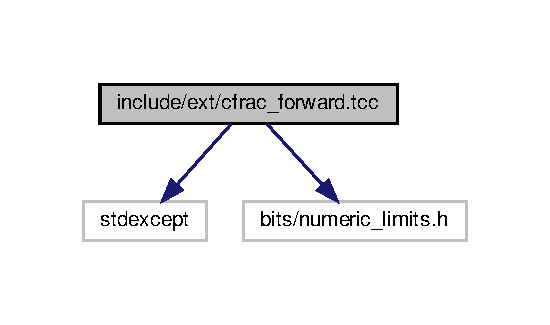
\includegraphics[width=264pt]{cfrac__forward_8tcc__incl}
\end{center}
\end{figure}
This graph shows which files directly or indirectly include this file\+:
\nopagebreak
\begin{figure}[H]
\begin{center}
\leavevmode
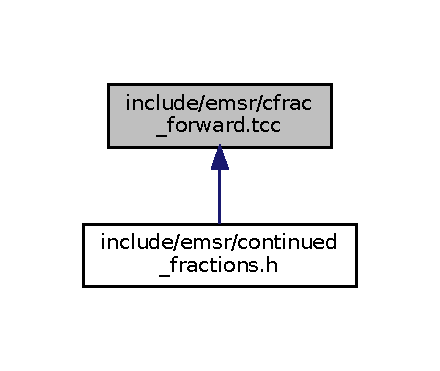
\includegraphics[width=223pt]{cfrac__forward_8tcc__dep__incl}
\end{center}
\end{figure}
\subsection*{Classes}
\begin{DoxyCompactItemize}
\item 
class \hyperlink{class__ForwardContinuedFraction}{\+\_\+\+Forward\+Continued\+Fraction$<$ \+\_\+\+Tp, \+\_\+\+A\+Fun, \+\_\+\+B\+Fun, \+\_\+\+Tail\+Fun $>$}
\end{DoxyCompactItemize}
\subsection*{Macros}
\begin{DoxyCompactItemize}
\item 
\#define \hyperlink{cfrac__forward_8tcc_a2ccccd967f8b9ade963c33f7e37572c3}{C\+F\+R\+A\+C\+\_\+\+F\+O\+R\+W\+A\+R\+D\+\_\+\+T\+CC}~1
\end{DoxyCompactItemize}


\subsection{Macro Definition Documentation}
\mbox{\Hypertarget{cfrac__forward_8tcc_a2ccccd967f8b9ade963c33f7e37572c3}\label{cfrac__forward_8tcc_a2ccccd967f8b9ade963c33f7e37572c3}} 
\index{cfrac\+\_\+forward.\+tcc@{cfrac\+\_\+forward.\+tcc}!C\+F\+R\+A\+C\+\_\+\+F\+O\+R\+W\+A\+R\+D\+\_\+\+T\+CC@{C\+F\+R\+A\+C\+\_\+\+F\+O\+R\+W\+A\+R\+D\+\_\+\+T\+CC}}
\index{C\+F\+R\+A\+C\+\_\+\+F\+O\+R\+W\+A\+R\+D\+\_\+\+T\+CC@{C\+F\+R\+A\+C\+\_\+\+F\+O\+R\+W\+A\+R\+D\+\_\+\+T\+CC}!cfrac\+\_\+forward.\+tcc@{cfrac\+\_\+forward.\+tcc}}
\subsubsection{\texorpdfstring{C\+F\+R\+A\+C\+\_\+\+F\+O\+R\+W\+A\+R\+D\+\_\+\+T\+CC}{CFRAC\_FORWARD\_TCC}}
{\footnotesize\ttfamily \#define C\+F\+R\+A\+C\+\_\+\+F\+O\+R\+W\+A\+R\+D\+\_\+\+T\+CC~1}


\hypertarget{cfrac__lentz_8tcc}{}\section{include/ext/cfrac\+\_\+lentz.tcc File Reference}
\label{cfrac__lentz_8tcc}\index{include/ext/cfrac\+\_\+lentz.\+tcc@{include/ext/cfrac\+\_\+lentz.\+tcc}}
{\ttfamily \#include $<$stdexcept$>$}\newline
{\ttfamily \#include $<$bits/numeric\+\_\+limits.\+h$>$}\newline
Include dependency graph for cfrac\+\_\+lentz.\+tcc\+:
\nopagebreak
\begin{figure}[H]
\begin{center}
\leavevmode
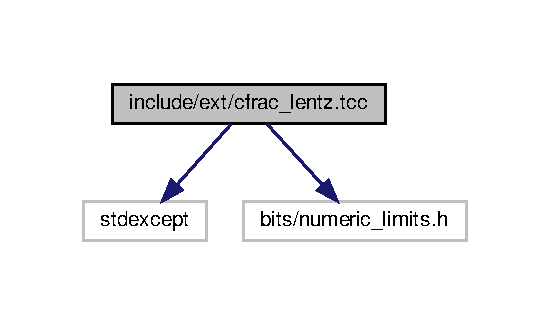
\includegraphics[width=264pt]{cfrac__lentz_8tcc__incl}
\end{center}
\end{figure}
This graph shows which files directly or indirectly include this file\+:
\nopagebreak
\begin{figure}[H]
\begin{center}
\leavevmode
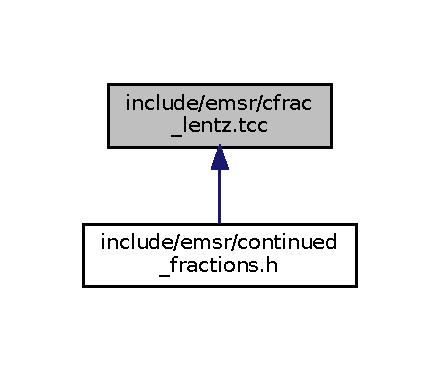
\includegraphics[width=211pt]{cfrac__lentz_8tcc__dep__incl}
\end{center}
\end{figure}
\subsection*{Classes}
\begin{DoxyCompactItemize}
\item 
class \hyperlink{class__LentzContinuedFraction}{\+\_\+\+Lentz\+Continued\+Fraction$<$ \+\_\+\+Tp, \+\_\+\+A\+Fun, \+\_\+\+B\+Fun, \+\_\+\+Tail\+Fun $>$}
\end{DoxyCompactItemize}
\subsection*{Macros}
\begin{DoxyCompactItemize}
\item 
\#define \hyperlink{cfrac__lentz_8tcc_a8763f0c1a80e6af178766a5908aa802b}{C\+F\+R\+A\+C\+\_\+\+L\+E\+N\+T\+Z\+\_\+\+T\+CC}~1
\end{DoxyCompactItemize}


\subsection{Macro Definition Documentation}
\mbox{\Hypertarget{cfrac__lentz_8tcc_a8763f0c1a80e6af178766a5908aa802b}\label{cfrac__lentz_8tcc_a8763f0c1a80e6af178766a5908aa802b}} 
\index{cfrac\+\_\+lentz.\+tcc@{cfrac\+\_\+lentz.\+tcc}!C\+F\+R\+A\+C\+\_\+\+L\+E\+N\+T\+Z\+\_\+\+T\+CC@{C\+F\+R\+A\+C\+\_\+\+L\+E\+N\+T\+Z\+\_\+\+T\+CC}}
\index{C\+F\+R\+A\+C\+\_\+\+L\+E\+N\+T\+Z\+\_\+\+T\+CC@{C\+F\+R\+A\+C\+\_\+\+L\+E\+N\+T\+Z\+\_\+\+T\+CC}!cfrac\+\_\+lentz.\+tcc@{cfrac\+\_\+lentz.\+tcc}}
\subsubsection{\texorpdfstring{C\+F\+R\+A\+C\+\_\+\+L\+E\+N\+T\+Z\+\_\+\+T\+CC}{CFRAC\_LENTZ\_TCC}}
{\footnotesize\ttfamily \#define C\+F\+R\+A\+C\+\_\+\+L\+E\+N\+T\+Z\+\_\+\+T\+CC~1}


\hypertarget{cfrac__steed_8tcc}{}\section{include/ext/cfrac\+\_\+steed.tcc File Reference}
\label{cfrac__steed_8tcc}\index{include/ext/cfrac\+\_\+steed.\+tcc@{include/ext/cfrac\+\_\+steed.\+tcc}}
This graph shows which files directly or indirectly include this file\+:
\nopagebreak
\begin{figure}[H]
\begin{center}
\leavevmode
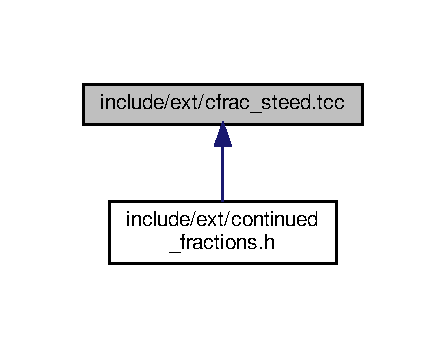
\includegraphics[width=214pt]{cfrac__steed_8tcc__dep__incl}
\end{center}
\end{figure}
\subsection*{Classes}
\begin{DoxyCompactItemize}
\item 
class \hyperlink{class__SteedContinuedFraction}{\+\_\+\+Steed\+Continued\+Fraction$<$ \+\_\+\+Tp, \+\_\+\+A\+Fun, \+\_\+\+B\+Fun, \+\_\+\+Tail\+Fun $>$}
\end{DoxyCompactItemize}
\subsection*{Macros}
\begin{DoxyCompactItemize}
\item 
\#define \hyperlink{cfrac__steed_8tcc_abc8003fbf1259def07f4af43fd210d99}{C\+F\+R\+A\+C\+\_\+\+S\+T\+E\+E\+D\+\_\+\+T\+CC}~1
\end{DoxyCompactItemize}


\subsection{Macro Definition Documentation}
\mbox{\Hypertarget{cfrac__steed_8tcc_abc8003fbf1259def07f4af43fd210d99}\label{cfrac__steed_8tcc_abc8003fbf1259def07f4af43fd210d99}} 
\index{cfrac\+\_\+steed.\+tcc@{cfrac\+\_\+steed.\+tcc}!C\+F\+R\+A\+C\+\_\+\+S\+T\+E\+E\+D\+\_\+\+T\+CC@{C\+F\+R\+A\+C\+\_\+\+S\+T\+E\+E\+D\+\_\+\+T\+CC}}
\index{C\+F\+R\+A\+C\+\_\+\+S\+T\+E\+E\+D\+\_\+\+T\+CC@{C\+F\+R\+A\+C\+\_\+\+S\+T\+E\+E\+D\+\_\+\+T\+CC}!cfrac\+\_\+steed.\+tcc@{cfrac\+\_\+steed.\+tcc}}
\subsubsection{\texorpdfstring{C\+F\+R\+A\+C\+\_\+\+S\+T\+E\+E\+D\+\_\+\+T\+CC}{CFRAC\_STEED\_TCC}}
{\footnotesize\ttfamily \#define C\+F\+R\+A\+C\+\_\+\+S\+T\+E\+E\+D\+\_\+\+T\+CC~1}


\hypertarget{continued__fractions_8h}{}\section{include/ext/continued\+\_\+fractions.h File Reference}
\label{continued__fractions_8h}\index{include/ext/continued\+\_\+fractions.\+h@{include/ext/continued\+\_\+fractions.\+h}}
{\ttfamily \#include \char`\"{}cfrac\+\_\+forward.\+tcc\char`\"{}}\newline
{\ttfamily \#include \char`\"{}cfrac\+\_\+lentz.\+tcc\char`\"{}}\newline
{\ttfamily \#include \char`\"{}cfrac\+\_\+steed.\+tcc\char`\"{}}\newline
Include dependency graph for continued\+\_\+fractions.\+h\+:
\nopagebreak
\begin{figure}[H]
\begin{center}
\leavevmode
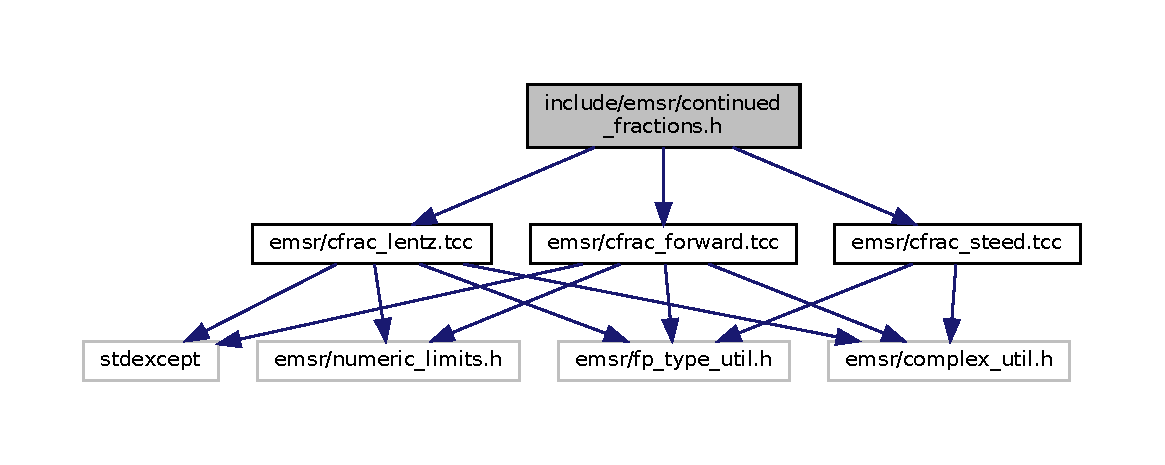
\includegraphics[width=350pt]{continued__fractions_8h__incl}
\end{center}
\end{figure}

%--- End generated contents ---

% Index
\backmatter
\newpage
\phantomsection
\clearemptydoublepage
\addcontentsline{toc}{chapter}{Index}
\printindex

\end{document}
